\documentclass[9pt,twocolumn,twoside]{gsajnl}
% Use the documentclass option 'lineno' to view line numbers

\articletype{inv} % article type
% {inv} Investigation 
% {gs} Genomic Selection
% {goi} Genetics of Immunity 
% {gos} Genetics of Sex 
% {mp} Multiparental Populations

\title{Kidney Renal Clear Cell Carcinoma expression analysis}

\author[$\ast$1]{Bofill A,}
\author[$\ast$1]{Castillo S,}
\author[$\ast$1]{Pérez A}


\affil[$\ast$]{Msc in Bioinformatics for Health Sciences, Pompeu Fabra University}

\keywords{Kidney; Carcinoma; Bioconductor}

\runningtitle{GENETICS Journal Template on Overleaf} % For use in the footer 

\correspondingauthor{Bofill}

\begin{abstract}

Renal Clear Cell Carcinoma is the most common type of Kidney cancer, but very few things are known about its molecular insights. In this  study, we perform a differential expression analysis coupled with a function enrichment analysis and a gene set enrichment analysis in order to identify the genes and paths that characterize  the molecular functioning of this type of cancer. We also build a Naive Bayes classifier to decide whether a sample is from a tumour or a normal tissue by their expression data. The results obtained indicate that renal clear cell carcinomas suffer a metabolic shift towards a strong fatty-acid synthesis by down-regulating their degradation and the oxidative phosphorilation. Results also single out PD-1 as a key factor for the immune system evasion of the tumour.


\end{abstract}
\setboolean{displaycopyright}{true}
\begin{document}
\maketitle
\thispagestyle{firststyle}
%\marginmark
\firstpagefootnote
\correspondingauthoraffiliation{Msc in Bioinformatics for Health Sciences, Pompeu Fabra University. adria.perez06@estudiant.upf.edu}
\vspace{-11pt}%


\section*{Introduction}

Kidney Renal Clear Cell Carcinoma (KIRC) is the most common type of kidney cancer (95\%) \citep{SEER}.  An estimated 62,700 new cases of kidney cancer are expected to be diagnosed in 2016, with 14.240 expected deaths (2,4\% of all death cancers).   The  5-year  and  10-year  relative  survival  rates  for  kidney  
cancer are 74\% and 62\% respectively.  Two-thirds of cases 
 are diagnosed at a local stage, for which the 5-year relative 
survival  rate  is  92\%, but when the tumour has spread from the kidney to other parts of the body, the rate lowers at 11\% \citep{SEER}. 


The renal clear cell carcinoma is a malignant cancer from the renal parenchyma, originated in the tubules. The clear cell carcinoma is one of the four major histologic subtypes, and the most common one (75\%). Clear cells are a specific cell-type defined by a clear cytoplasm due to a high lipid content. This subtype is the least likely to reproduce, but has a strong resistance to chemotherapy and radiotherapy. The primary treatment is nephrectomy or partial nephrectomy, and sometimes laparoscopic techniques are used. 
	

Although KIRC is a common cancer, little has been done to its molecular characterization. The reason behind its high resistance to chemotherapy and radiotherapy is still unknown. Some molecular alterations have been identified. The PI3K/AKT pathway seems to be recurrently mutated, and a widespread DNA hypomethylation was associated with a mutation of the \textit{SETD2} methyltransferase. In some cancers, there's evidence of a methabolic shift, with down-regulation of the oxidative phosphorylation  and the fatty-acid degradation pathways and up-regulation of the pentose phosphate pathway \citep{Creighton2013}.

A molecular characterization of the KIRC is needed in order to identify the key molecular mechanisms that cause this cancer and target them in novel treatments. In this study,  a differential expression analysis of the RNA-Seq data provided by the The Cancer Genome Atlas (\href{http://www.cancergenome.nih.gov}{TCGA}) has been performed, with a further functional enrichment analysis of GO/KEGG terms and a Gene Set Enrichment Analysis (GSEA) to identify the molecular profile of this cancer.

\section*{Materials and Methods}
\subsection*{Data characterization}
The Kidney Renal Clear-Cell Carcinoma RNA-seq data used in this study has been extracted from TCGA. The initial data available from TCGA dataset comprised 542 tumours and 72 normal samples. The tumour group include 187 females and 337 males, while the normal one is formed by 20 female and 52 males. Analysing this data samples, 38 paired samples were found. Each sample has a total of 20115 genes. 

\newcolumntype{b}{X}
\newcolumntype{s}{>{\hsize=.5\hsize}X}
\begin{table*}[htbp]
\centering
\caption{\bf Five most over-represented Biological Process GO terms in over-expressed genes in KIRC. }
\begin{tableminipage}{\textwidth}
\begin{tabularx}{\textwidth}{ssssssb}
\hline
GOBPID & Pvalue & OddsRatio & ExpCount & Count & Size & Term\\
\hline
GO:0051301 & 0.000 & 1.534 & 165 & 206 & 402 & cell division\\
GO:0051251 & 0.000 & 2.064 & 54 & 77 & 131 & positive regulation of lymphocyte activation\\
GO:0007156 & 0.000 & 2.469 & 35 & 53 & 84 & homophilic cell adhesion via plasma membrane adhesion molecules\\
GO:0008283 & 0.000 & 1.275 & 459 & 518 & 1117 & cell proliferation\\
GO:0032946 & 0.000 & 2.634 & 27 & 42 & 65 & positive regulation of mononuclear cell proliferation\\
\hline
\end{tabularx}
%  \label{tab:shape-functions}
\end{tableminipage}
\label{table:1}
\end{table*}

\subsection*{Statistics and data analysis}
All the analyses have been performed with R. You could find more information about that in: \url{www.r-project.org}. We have used the \href{https://bioconductor.org/packages/release/bioc/html/edgeR.html}{EdgeR} \citep{Robinson2010} package from \href{https://bioconductor.org}{Bioconductor} \citep{Gentleman2004}  for the differentially expressed gene identification analysis.

\subsubsection*{Quality and normalization }
: The library size of the samples has been analysed and major differences in sequencing depth were found. We filtered out the samples with a low sequencing depth (< 45 Millions per read). We obtained a filtered dataset of 298 tumour and 48 normal samples. To obtain a more accurate information and to reduce the size of our set, we determined to use a paired design, taking into account the patient variability. For this reason, we only considered the 38 paired samples for the further analyses.

To filter out the genes with a low or without expression, we analysed the distribution of expression levels among genes using the log Counts Per Millions measure (logCPM). (GRAFICA? S7). We determined a cut-off of 1 logCPM. With this filter we reduce the number of genes from 20,115 to 12,495 genes.

The Trimmed Mean of M-values method (TMM) \citep{Robinson2010}, implemented in the EdgeR package, was used to normalize the expression values.

Analysing MA-plots \citep{Dudoit2002}, a normal sample (TGCA-CW-5591) was found to have an abnormal major gene expression bias in the association between the fold-changes and average expression, resulting in a large dependence between both variables of the MA plot. For this reason, this sample and its paired in the tumour set were removed from the analysis.


\subsubsection*{Batch Effect Analyses}
: Four possible sources of variation were considered for the batch effect identification \citep{Leek2010}: Gender, Tissue Source Site (TSS), Plate, and portion analyte. For each one of these batch indicators, we performed a hierarchical clustering using the Spearman correlation coefficient citep{Spearman1904}  and a multidimensional scaling plot, in order to assess their possible effect. We conclude that none of them confound the primary source of variation, which in this case is the cell-type (tumour/normal).

\subsubsection*{Differential expression analysis	}
: To perform the differentially expressed gene identification analysis, we generate a two factors linear model, taking into account the cell-type variable (normal/tumour type) and the patient \citep{Smyth2004}.

We modelled the mean variance trend of logCPM values, computing the weights of this relationship at the individual observation level. In order to perform this part, we applied the voom function, implemented in the \href{https://bioconductor.org/packages/release/bioc/html/limma.html}{limma R-package}, which is part of the BioConductor project. A Surrogate Variable Analysis (SVA) was performed to identify the possibles sources of variation that are not related with our variables of interest (cell-type)  \citep{Leek2007}.

After fitting the data to the linear model, we applied the empirical Bayes approach (eBayes) that should result in a far more stable inference. A False Discovery Rate (FDR)) \citep{Benjamini1995} cut-off of 0.01 was applied to classify the genes as over-expressed, under-expressed or without changed in expression. In order to reduce the number of differentially expressed genes, we classified the genes in two further groups: strongly over-expressed, using a log Fold-changes cut-off of 5 (logFC > 5), and strongly under-expressed (logFC < -5). 

\subsubsection*{Functional Enrichment}
: A Gene Ontology analysis (\href{http://geneontology.org}{GO}) and Kyoto Encyclopedia of Genes and Genomes (\href{http://www.genome.jp/kegg/}{KEGG}) analyses were performed with the differentially expressed genes set. Fisher's exact test \citep{Fisher1922} was applied to obtain the most representative biological process gene ontology terms or KEGG pathways (P< 0.01). The significance of the GO terms is computed conditionally to the significance of its child terms \citep{Alexa2006}. The enrichment tests were performed in three different gene sets: the whole list of differentially expressed genes, the over-expressed gene set and the under-expressed gene set. The GO and KEGG results are available in the supporting materials together with the raw p-values.

\subsubsection*{Gene Set Enrichment Analysis}
:  Using \href{http://bioconductor.org/packages/release/bioc/html/GSEABase.html}{GSEABase package} from the BioConductor project, the Simple Gene Set Enrichment Analysis (GSEA) algorithm \citep{Subramanian2005, Irizarry2009} was applied in order to assess differences in  expression at the pathway level. We used the data set called c2BroadSets from the \href{https://bioconductor.org/packages/release/data/experiment/html/GSVAdata.html}{GSVAdata} to obtain the different gene sets, restricting the pathways to the ones from \href{http://www.genome.jp/kegg/}{KEGG} , \href{http://www.reactome.org}{REACTOME} and \href{http://www.genecarta.com}{BioCarta}. We used an FDR < 1\% to call the pathways differentially expressed.

\begin{figure}[htbp]
\centering
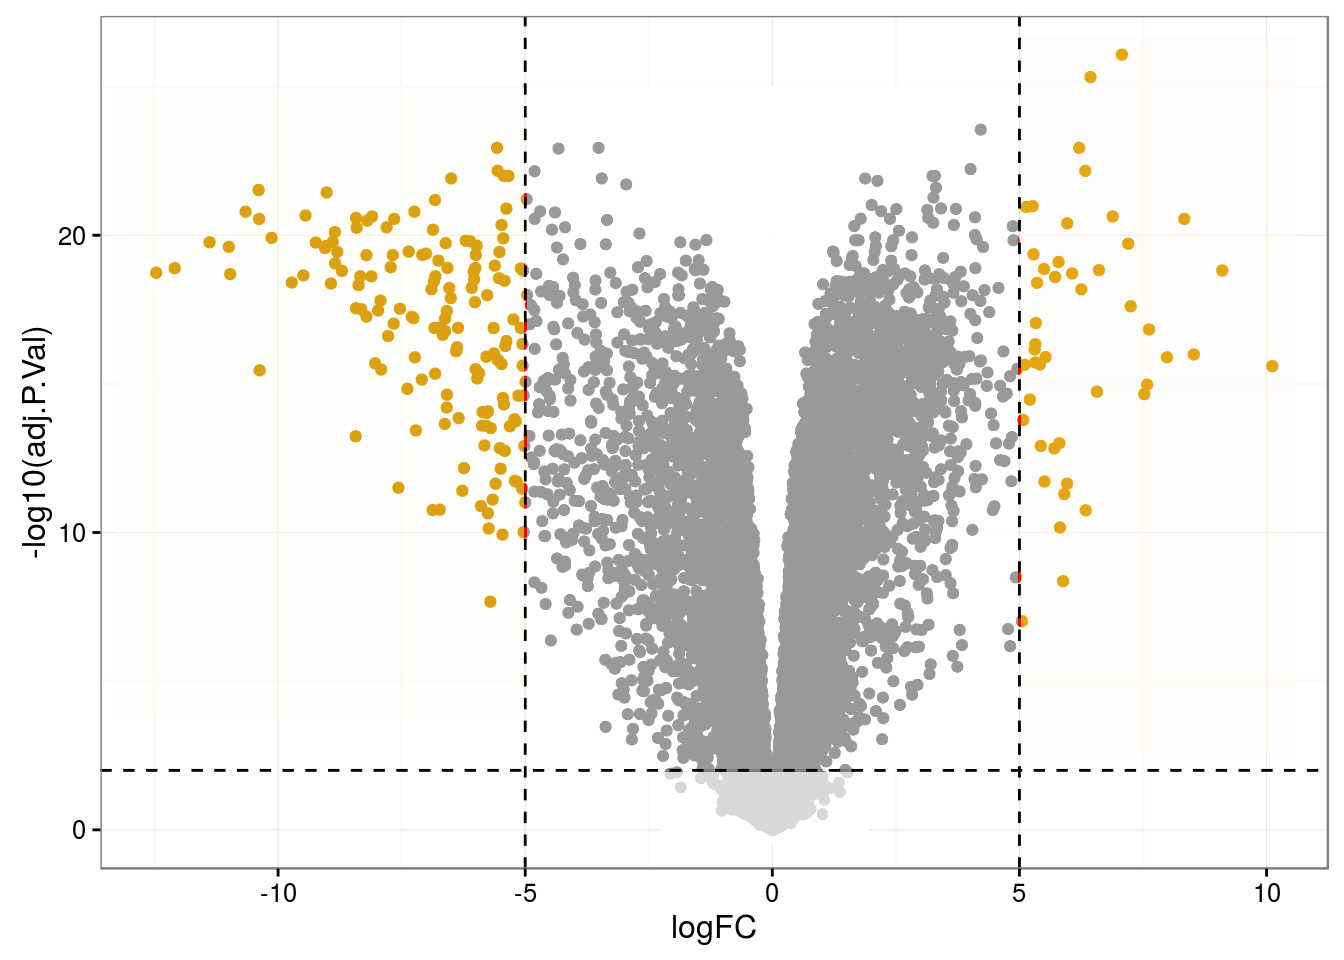
\includegraphics[width=\linewidth]{figures/fig1_volcano.png}
\caption{Volcano plot of the differential expression analysis of Kidney Renal Clear Cell Carcinoma. The horizontal dashed line represents the FDR cut-off of 0.01 used for calling DE genes. After calling 9,108 genes as DE, we reduced the number of genes using a Fold Change cutoff of 5 and -5 (vertical lines), resulting in two groups of strongly over-expressed and strongly under-expressed genes (in yellow). }%
\label{fig:volcanoplot}
\end{figure}

\subsubsection*{Hierarchical Clustering and Naive Bayes classifier}
: We used the strongly over-expressed genes and under-expressed genes, a total of 199 genes, to determine if these genes alone are able to separate our samples in two clusters using a Hierarchical Clustering approach \citep{Spearman1904}. This approach has been applied over the 38 paired samples and also over the whole set of samples (614 samples).

Applying the R package \href{https://cran.r-project.org/web/packages/e1071/index.html}{e1071}, a Naive Bayes Classifier was generated, using the paired samples as the training set, considering only the 199 strongly DE genes as features. This classifier was used to predict the cell type of the remaining 540 samples. 

\subsection*{Data Availability}

The full workflow of our analysis is given in a supplementary HTML file. The file was generated with R, using markdown. It contains the script used, along with explanations and interpretations in every step and complementary figures generated during the analysis to give an informative display of our data.  


\section*{Results and Discussion}
\subsection*{Differentially Expressed Analysis}
The DE analysis shows 9,108 differentially expressed genes in KIRC tumour, being 4,014 under-expressed and 5,094 over-expressed. Out of these DE genes, 46 were classified as strongly over-expressed and 153 as strongly under-expressed. The volcano plot represented in (Fig. \ref{fig:volcanoplot}) shows the different filters applied to the whole set of genes.

Analysing individual genes previously found to be mutated in the KIRC development, the chromatin regulators SETD2 and PBRM1 are over-expressed, even though they are tumour-suppressor genes as they promote a correct chromatin remodelling and DNA repair \citep{Creighton2013, Kanu2015}. While PI3K/AKT pathway has been targeted as strong therapeutical target \citep{Creighton2013}, we did not find any over-expressed gene of this pathway (PTEN/PI3K/PDK1/AKT/MTOR).

\subsection*{Functional Enrichment}
The Functional Enrichment analysis using GO terms revealed 96 over-represented terms and 59 under-represented [Full results here and here]. The most representative terms in the over-represented group include cell-division and proliferation, intrinsic properties in any malignant cell. 

Another group of representative terms are the ones related with regulation of immune response and T-cell functioning. This suggests that KIRC may cause a huge deregulation of the local immune response to the tumour. 

When looking at the under-represented terms, many of them are related with renal function like ion transport and small molecule metabolism. Several terms related with the oxidative phosphorilation pathway are under-represented along with fatty-acid degradation. This metabolical shift to fatty-acid synthesis and inactivation of oxidative phosphorilation was previously identified in KIRC \citep{Creighton2013}.

\begin{figure}[htbp]
\centering
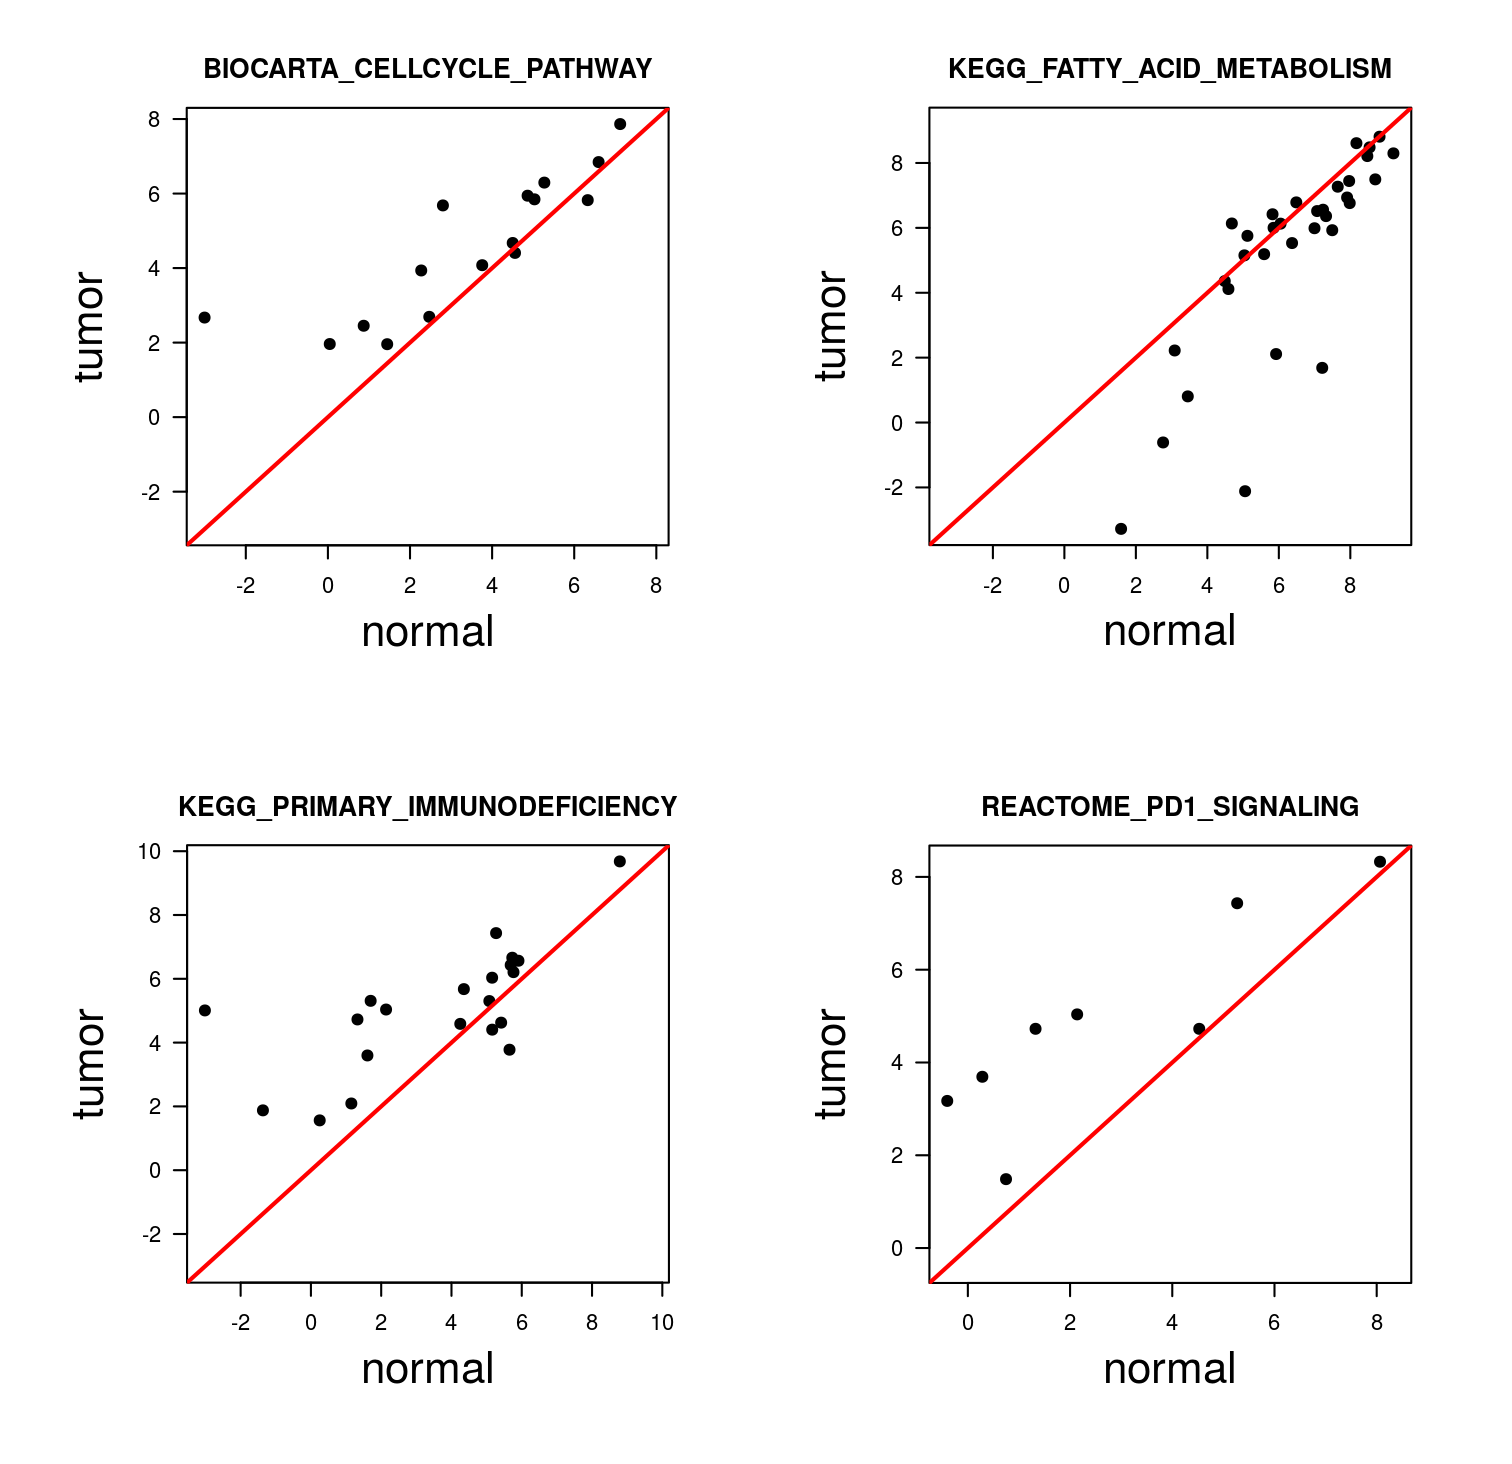
\includegraphics[width=\linewidth]{figures/fig3.png}
\caption{Highlighted gene sets/pathways differentially expressed in KIRC. After performing a Simple GSEA, many gene sets from KEGG, REACTOME and BioCarta were found to be differentially expressed. In this plot we have represented four of them, comparing the normalized logCPM for normal and tumour samples. From left to right and top to bottom, the pathways are: cell cycle pathway, fatty acid metabolism, primary immunodeficiency and PD-1 signalling.}%
\label{fig:pathways}
\end{figure}


KEGG analysis results show that among the most represented pathways over the over-expressed DE genes, some KEGG pathways terms related to the immune system response, such as primary immunodeficiency and T-cell receptor signalling pathway, can be found.  These results are in line with the suggested hypothesis of an immune system deregulation in KIRC. Furthermore, the p53 signalling pathway is also found as one of the most over-represented pathways.

On the other hand, oxidative phosphorylation and fatty acid degradation are found to be among the most represented pathways over the under expressed DE genes. As seen with the GO terms, this indicates a metabolic shift in KIRC to promote fatty acid synthesis and inactivates the oxidative phosphorylation.


\begin{figure*}[htbp]
\centering
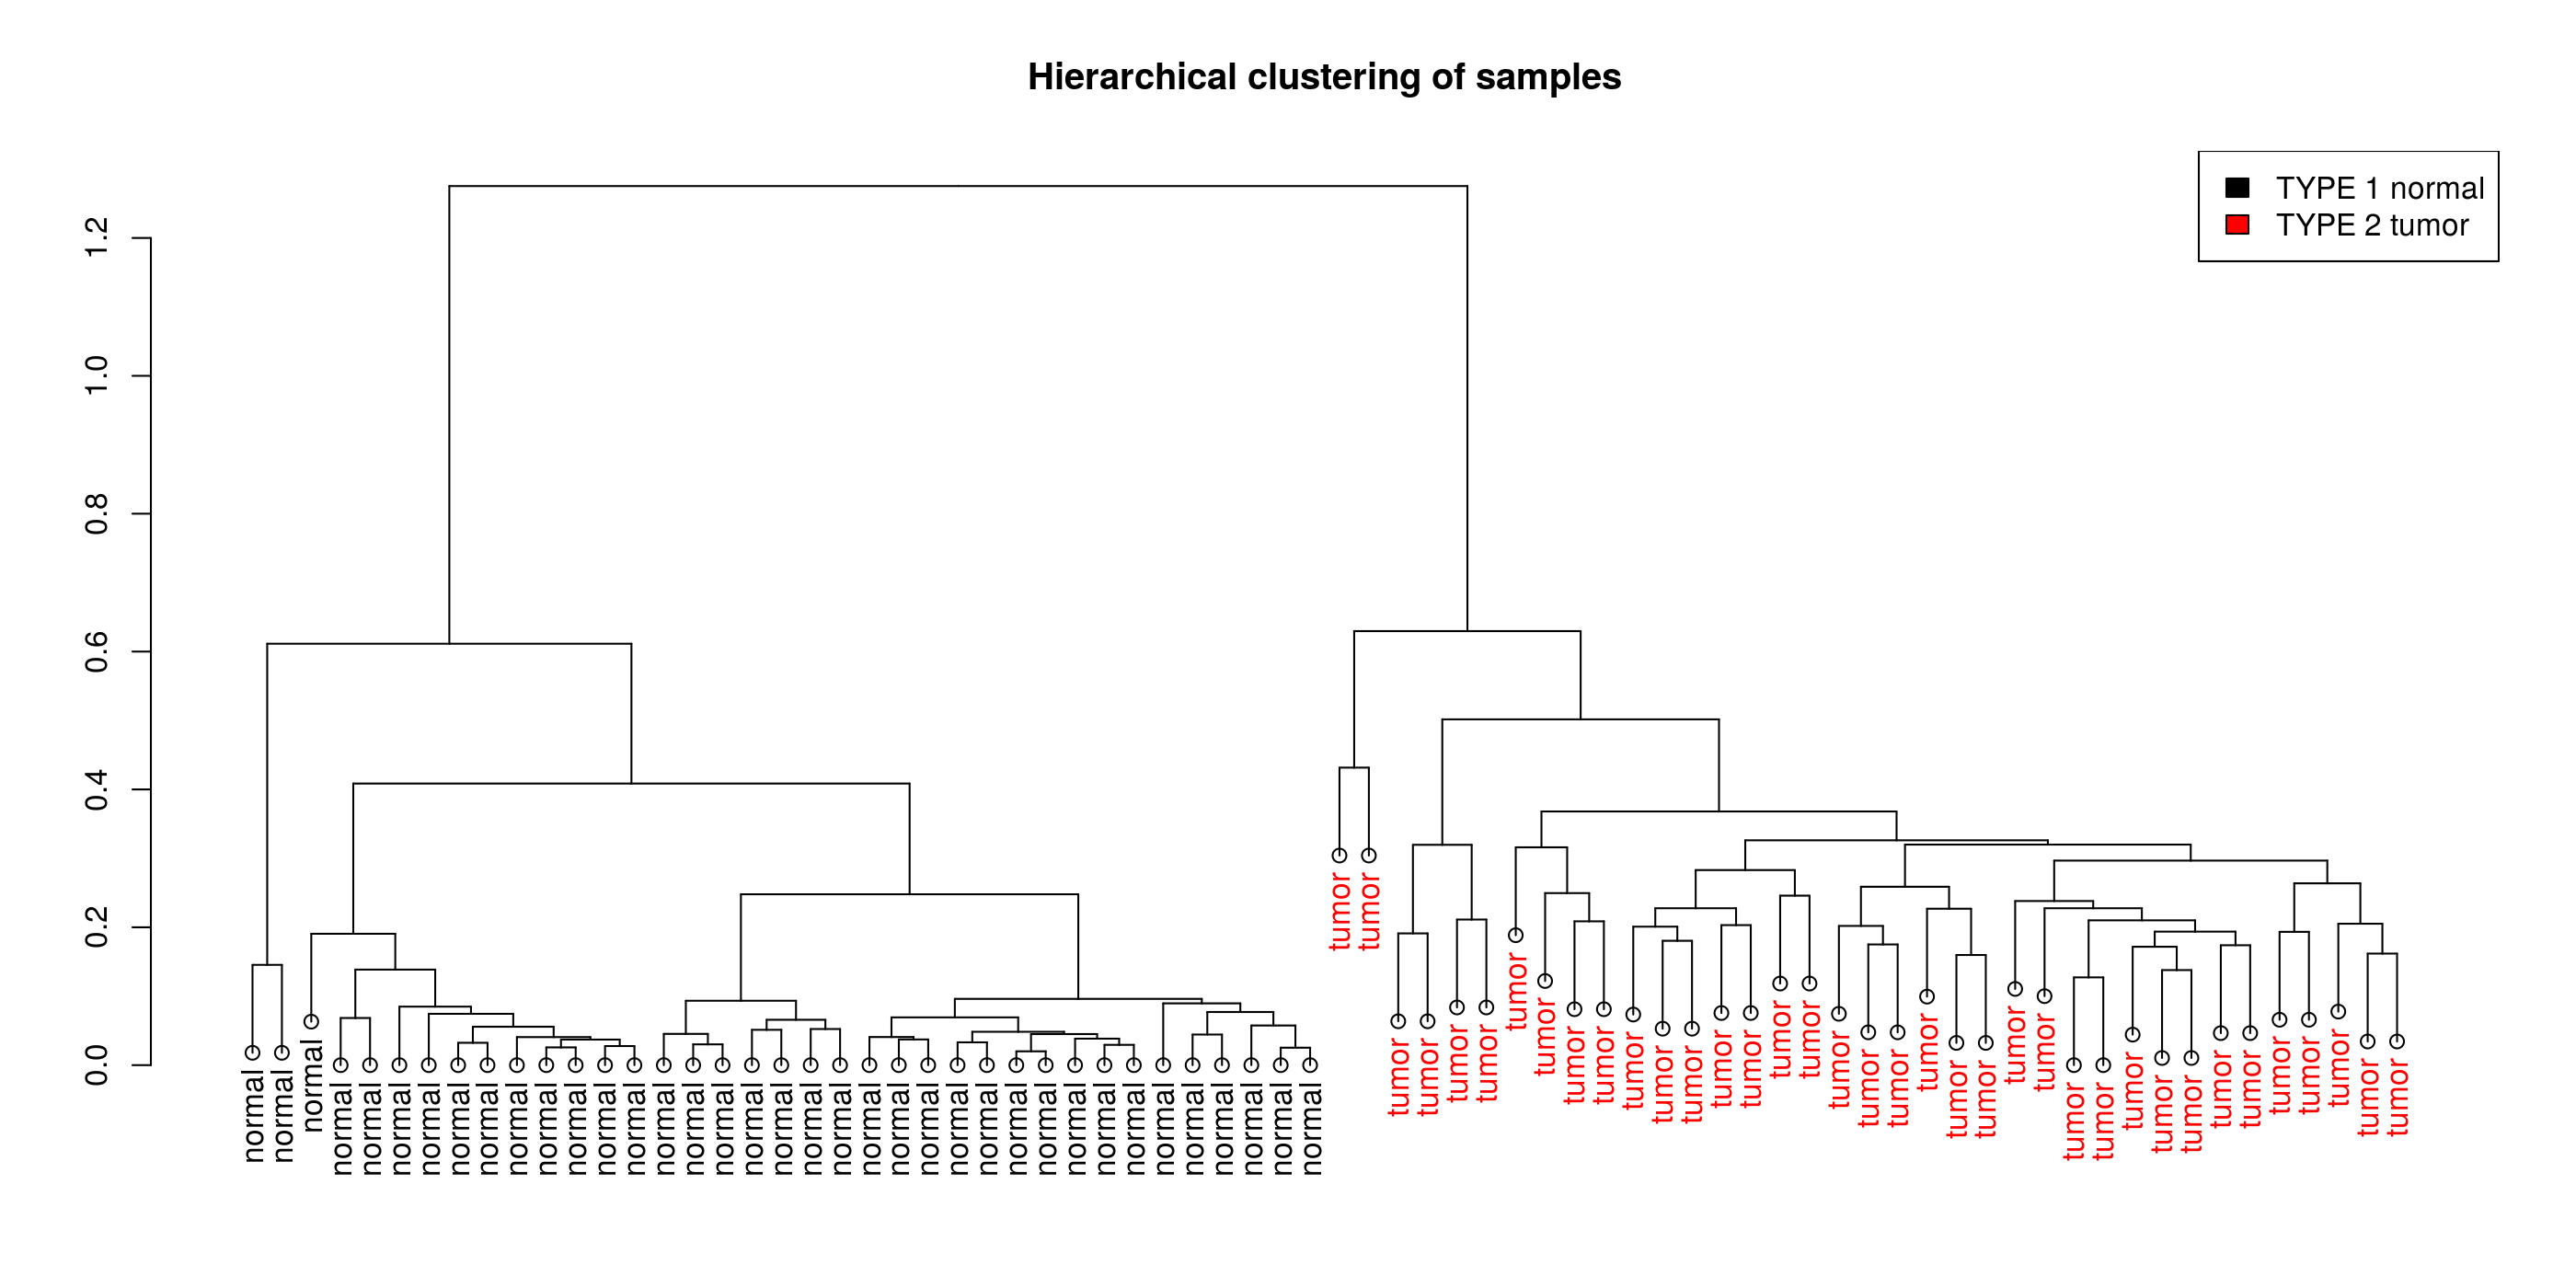
\includegraphics[width=\textwidth]{figures/fig2.png}
\caption{Hierarchical clustering of paired samples using the 199 differentially expressed genes in KIRC. After calling the DE genes using an FDR of 1\%, all the samples used for this expression study were clustered by means of the Spearman's correlation coefficient, but reducing the feature vector to only the logCPM of the differentially expressed genes. }%
\label{fig:hierarchical}
\end{figure*}


\subsection*{Gene Set Enrichment Analysis}
The GSEA results show 677 DE pathways. In this study we only focused on the top ones. This results can be found on supplementary materials (Fig. S22).

The analysis highlights again the loss of kidney function and the metabolic shift to the fatty acid synthesis  (Fig. \ref{fig:pathways}). We found several pathways of small molecules, cation and glucose transport across the membrane that are under-expressed in KIRC, suggesting that the renal function is disrupted. As seen before in the Functional Enrichment analysis results, we found the oxidative phosphorilation and the fatty acid degradation pathways under-expressed, indicating an increase of fatty acid synthesis and  an inactivation of the TCA cycle in favour of the pentose phosphate pathway, as suggested in \citep{Creighton2013}. 

As previously mentioned in the Functional Enrichment results, many immune system sets are found to be differentially expressed. Primary immunodeficiency, T-cell apopotosis and PD1 signalling pathways, show us clues of how KIRC evades the immune function of the organism. The BioCarta T-cell apoptosis pathway is characteristic of the HIV infection and describes how the virus induces T-cell apoptosis. The fact that KIRC presents this feature indicates that this may be an useful mechanism for this tumour to not be recognized as a malignant cell.


Programmed Cell Death Protein 1 (PD-1/CD279) is a cell surface receptor that belongs to the immunoglobulin super-family and is expressed in T-cells. It functions as an immune checkpoint, negatively regulating the immune response \citep{Francisco2010}. PD1 plays an important role in down-regulating the immune system, reducing autoimmunity and promoting self-tolerance through the induction of antigen-specific T-cell apoptosis.
PD-1 has been involved in the tumour cell evasion of the host immune system \citep{Iwai2002}. This argument is in line with the over-expression of PD-1 found in our GSEA results. This protein has been proposed as target for several drugs that are currently in different trial stages, such as Nivolumab, used as a possible second line treatment for renal cell carcinoma \citep{nivolumab}.


\subsection*{Naive Bayes classifier}
With a Hierarchical Clustering approach, we can observe if the strongly DE genes separate the samples in different clusters. We applied this method to the paired samples and we can observe a clear separation between normal and tumour samples in two clusters (Fig. \ref{fig:hierarchical}). 

The application of this approach to the whole set of samples results in a more complex set of clusters. Although almost the entire set of normal and tumour samples cluster together, some tumour samples show an unexpected clustering behaviour (Fig. S24). These samples are closer to the cluster of normal samples, leading us to determine that these strongly DE genes do not capture the whole variability between tumour and normal samples.

With the Naive Bayes Classifier, over the prediction of the cell type of the unpaired samples, we computed the specificity and sensitivity and we obtain a value of 0.971 and 0.921 respectively. The F-measure computed with these values results in a value of 0.0609. In  \citealt{Yang2014} , a similar classifier was built, but using a Support Vector Machine instead of a Naive Bayer Classifier. Although K-Fold Cross Validation was not done in our study, which could explain the differences in the evaluation of the effectiveness of this classifier, the specificity and sensitivity results are very similar.

\section*{Conclusions}

Performing a general DE analysis coupled with functional enrichment and gene-set enrichment analysis has provided us with a decent characterisation of the renal clear cell carcinoma. We have been able to single out the differentially expressed genes in this type of cancer, and analyse this data to pinpoint the main molecular pathways that lead to cell malignancy in KIRC. 

The analysis has identified the main metabolic route of the tumour, promoting the fatty-acid synthesis and inhibiting the oxidative phosphorilation, validating the histological feature of a clear cytoplasm in clear cells. It has also spotted PD-1 signalling pathway as a major tool to evade the immune system, and
stood out a general immune evasion and down-regulation from the tumour.

This results help us to establish putative targets for pharmacological treatment, in order to improve the current treatments. PD-1 has been identified as an important target for cancer immunotherapy, activating the immune system to attack malignant cells, and the PD-1 inhibitor Nivolumab \citep{nivolumab} has been used to treat renal cell carcinoma.


This demonstrates how our analysis was able to identify a target protein that has drug inhibitors already in clinical trials, reinforcing our  methodology as a system to molecularly characterize tumours and point out putative targets to address cancer treatments.

\bibliography{example-bibliography}

\end{document}